\documentclass[10pt, a4paper]{report}

\usepackage[utf8]{inputenc}
\usepackage{polski}
\usepackage{a4wide}
\usepackage{fancyhdr}
\usepackage{lastpage}
\usepackage{tabularx}
\usepackage{listings}
\usepackage{graphicx}

\graphicspath{ {./images} }

%strona tytułowa
\begin{titlepage}

\title{\huge{\textbf{Sprawozdanie}}\\ gramatyk bezkontekstowych}
\author{Szymon Półtorak}
\date{}

\end{titlepage}

\renewcommand{\footrulewidth}{1pt}

\begin{document}
    \maketitle

    \renewcommand*\thesection{\arabic{section}} 
    
    \pagestyle{fancy}
    \fancyhf{}
    \rhead{Szymon Półtorak}
    \cfoot{Strona \thepage \hspace{1pt} z \pageref{LastPage}}
    
    \fancypagestyle{plain}{
        \rhead{Szymon Półtorak}
        \cfoot{Strona \thepage \hspace{1pt} z \pageref{LastPage}}
    }
    \tableofcontents
    \newpage

    \section{Treść Zadania}
    
    \begin{figure}[h]
        \begin{center}
            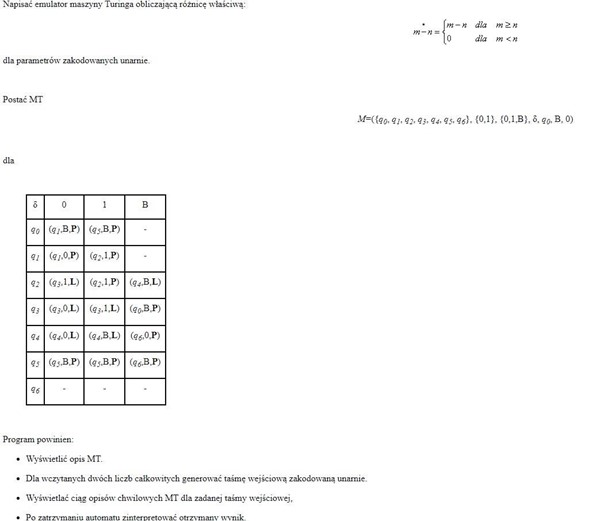
\includegraphics[scale=0.9]{photo1.jpg}
            \caption{Treść zadania}
        \end{center}
    \end{figure}
    \newpage

    \section{Instrukcja Obsługi Programu}
    Żeby uruchomić program trzeba wejść w program Visual Studio 2019 Enterprise i po załadowaniu projektu trzeba wybrać
    opcję „Local Windows Debugger”.

    \begin{figure}[h]
        \begin{center}
            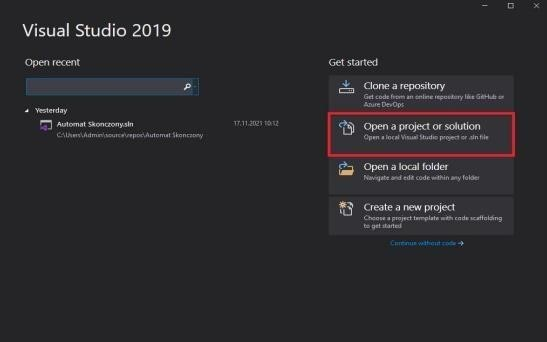
\includegraphics[scale=1]{photo2.jpg}
            \caption{mportowanie Projektu}
        \end{center}
    \end{figure}

    Po uruchomieniu programu wyświetli nam się opis Maszyny Turinga. Poprosi on nas o podanie liczb potrzebnych do
    wykonania (m i n). Po podaniu tych informacji program wyświetli ciąg opisów chwilowych oraz wynik odejmowania. Maszyna
    Turinga nie obsługuje liczb ujemny, dlatego dla każdego m < n wypisze wynik równy 0. Program poczeka na użycie dowolnego
    przycisku i zakończy działanie.

    \begin{figure}[h]
        \begin{center}
            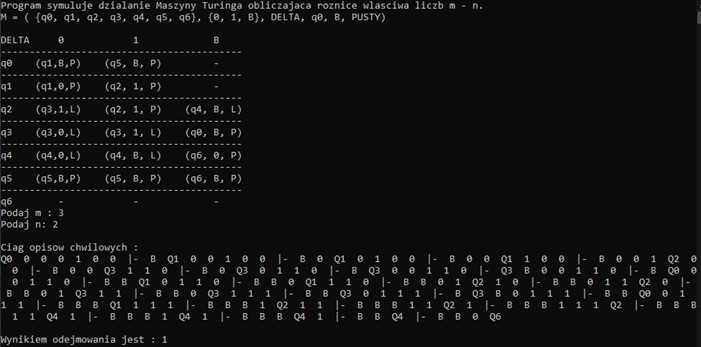
\includegraphics[scale=0.8]{photo3.jpg}
            \caption{Przykładowe wywołanie}
        \end{center}
    \end{figure}

    \newpage

    \section{Przykładowe wywołania dla m = 2 i n = 1 oraz m = 1 i n = 2}
    a) m = 2, n = 1
    Właściwe działanie Maszyny Turinga: 
    \begin{lstlisting}
    Q0 0 0 1 0 |- B Q1 0 1 0 |- B 0 Q1 1 0 |- B 0 1 Q2 0 |- B 0 Q3 1 1 
    |- B Q3 0 1 1 |- Q3 B 0 1 1 |- B Q0 0 1 1 |- B B Q1 1 1 |- B B 1 Q2 1 
    |- B B 1 1 Q2 B  |- B B 1 Q4 1 B |- B B Q4 1 B B 
    |- B Q4 B B B B |- B 0 Q6 B B B         
    \end{lstlisting}

    \begin{figure}[h]
        \begin{center}
            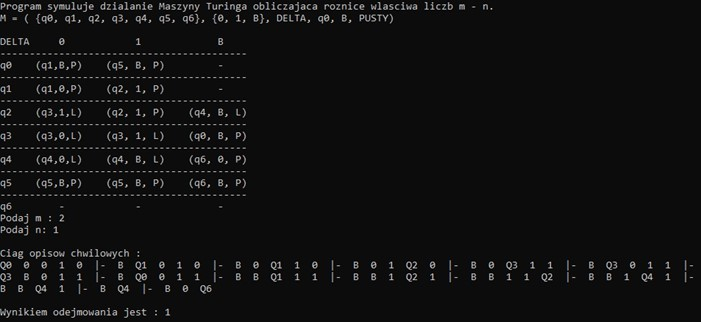
\includegraphics[scale=0.8]{photo4.jpg}
            \caption{ Wyświetlony wynik działania programu}
        \end{center}
    \end{figure}
    \newpage
    Wynik odejmowania podany przez program: 1
    \newline\newline b) m = 1, n = 2
    Właściwe działanie Maszyny Turinga: 
    \begin{lstlisting}
    Q0 0 1 0 0 |- B Q1 1 0 0 |- B 1 Q2 0 0 |- B Q3 1 1 0 
    |- Q3 B 1 1 0 |- B Q0 1 1 0 |- B B Q5 1 0
    |- B B B Q5 0 |- B B B B Q5 B |- B B B B B Q6 B        
    \end{lstlisting}

    \begin{figure}[h]
        \begin{center}
            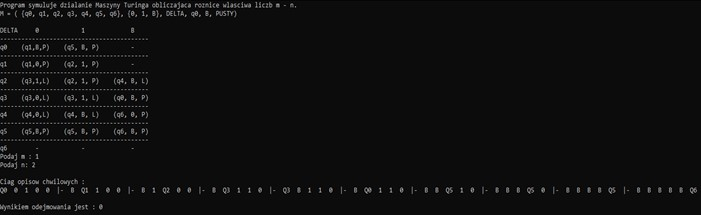
\includegraphics[scale=0.8]{photo5.jpg}
            \caption{ Wyświetlony wynik działania programu}
        \end{center}
    \end{figure}
    Wynik odejmowania podany przez program: 0 

    \section{Bibliografia}
    \begin{enumerate}
        \item \textit{Język ANSI C}, Brian W. Kernighan, Dennis M. Ritchie,
        \item \textit{Wprowadzenie do teorii automatów, języków i obliczeń}, John Hopcroft, Jeffrey Ullman.
    \end{enumerate}

\end{document}